\documentclass[a4paper,english]{ifimaster/ifimaster}
\usepackage[utf8]{inputenc}
\usepackage{babel,duoforside/duomasterforside}
\usepackage[hidelinks]{hyperref}
\usepackage{comment}
\usepackage{xcolor}
\usepackage{graphicx}
\usepackage{parskip}

% \usepackage[hyphens]{url}
% \usepackage[hidelinks]{hyperref}
% \hypersetup{breaklinks=true}
% \urlstyle{same}

% \usepackage[backend=biber,style=authoryear]{biblatex}
% \addbibresource{citations.bib}



\newcommand{\AAcomment}[1]{\textcolor{green}{#1}}
\newcommand{\MGcomment}[1]{\textcolor{red}{#1}}
\newcommand{\AScomment}[1]{\textcolor{blue}{#1}}



\title{Title}
\subtitle{Sub-title}
\author{Ahmed Abdulrahman Hussein Abbas}

\begin{document}
\duoforside[dept={Department of Informatics},
program={Informatics: Programming and System Architecture},
long]

\frontmatter{}
\chapter*{Abstract}

OptiqueVQS is a visual query system which allows the users to easily construct complex queries over data described by an ontology. However complex queries over a large dataset are very expensive and time consuming. User interfaces which adjust based on the available underlying data usually improve the user experience. So queries which lead to no answers are undesirable since they waste the user's time. 

Dead-end detection is a very common approach to effectively detecting and preventing a user from choosing an extension that will lead to a query with no answers. However the standard approach to detecting dead-ends is often too inefficient since it requires querying over the data, but with too large datasets this is infeasible. A solution to this problem is to do approximate dead-end detection which uses an index-based framework.

For optimal performance, we need a fast implementation of the index. In this essay, we'll explain the problem, discuss different solutions with search engines and how we can use a search engine like Elasticsearch to store the index and implement a solution to the problem that we have. In the end we'll look at how we can extend the work in several directions. 

\chapter*{}

\chapter*{Acknowledgements}

I would like to thank my supervisors, Martin Giese, Ahmet Soylu and Vidar Norstein, ...

\chapter*{}

\tableofcontents{}

\chapter*{}

\listoffigures{}
\listoftables{}


\mainmatter{}
\chapter{Introduction}

\section{Problem Description} \label{Problem description}

In OptiqueVQS we show a visual representation of the partially constructed query, and present the domain implicitly by providing lists of valid modifications to the constructed query. From this, the user can select an extension to make a new version of the query. This extension process is repeated until the user is satisfied, and after that, they can run the final query over the dataset.~\cite{vidar-phd-2020}

In addition to showing the users lists of valid modifications to the constructed query, we are interested in showing the users if a query returns no answers when the user is searching for a non-empty subset of the data. To be able to do this, we have to effectively detect and prevent a user from choosing an extension that will lead to a query with no answers. Basically we want to make a system that is able to detect \textit{dead-end extensions}. 

\begin{figure}[htp]
    \centering
    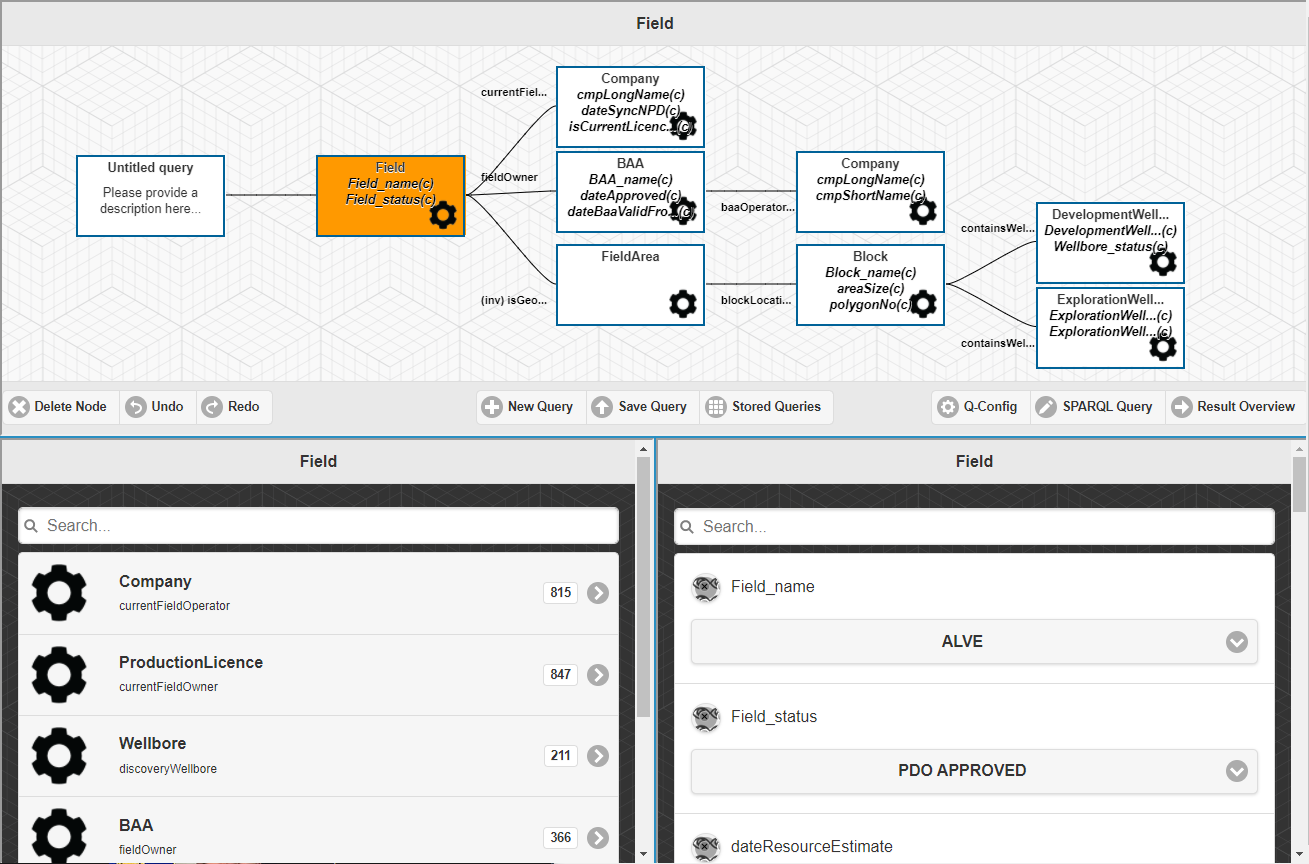
\includegraphics[width=12cm]{images/optiqueVQS.PNG}
    \caption{OptiqueVQS}
    \label{fig:optiqueVQS}
\end{figure}

Dead-ends detection is actually quite common in the search paradigm used by most e-commerce websites, known as faceted search. In general, dead-ends can be found by simply executing the queries generated by each of the possible extensions, and flag those where the corresponding result is empty. But, unless the database is optimized for these kinds of queries, this process could take minutes, which is not acceptable because it interrupts the user’s workflow which is not good for user usability.~\cite{vidar-phd-2020} 

However a solution to this problem is to use index-based searching engines like Elasticsearch, but these engines have a more limited query expressivity where they only support queries over one single class. OptiqueVQS supports queries over multiple classes, where the query may consist of multiple connected classes. 

In the thesis \textit{Adaptive Query Extension Suggestions for Ontology-Based Visual Query Systems}~\cite{vidar-phd-2020} a flexible framework for caching and indexing that precomputes much of the information required to produce adaptive suggestions in the user interface was presented. The idea behind the framework is that since in OptiqueVQS we allow queries with arbitrarily many connected classes, an index to support every such query would need to be infinitely large. So instead we can use approximations that detect most dead-ends since it's not really possible to guarantee both efficient and complete dead-end detection using a finite amount of memory. This approximation method can be achieved by only considering certain essential subsets of the data, which then only requires a finite index. To determine which parts of the data to include in the index we use a configuration structure.~\cite{vidar-phd-2020, VQS_search} 


The goal is to have a working implementation of a \textit{dead-end preventing extensions system} that will detect dead-ends. Since queries to the index only concern a single table, we are interested in implementing the approach using a search engine as index storage, like Elasticsearch to build fast and scaleable backend support for the query interface. This should make it possible to scale up index storage over a cluster. An additional benefit of using a search engine like Elasticsearch is that it also supports approximate text search, quick completion of text entry fields, etc.~\cite{vidar-phd-2020, VQS_search} 

\section{Motivation}

\section{Related and Previous Work}

\section{Thesis Structure}

\textbf{Chapter 2} is an overview of the background theories and tools that will be useful when we later present the main work of the thesis.


\noindent \textbf{Chapter 3} is an ...

\noindent \textbf{Chapter 4} is an ...

\noindent \textbf{Chapter 5} is an ...

\noindent \textbf{Chapter 6} is an ...

\noindent \textbf{Chapter 7} is an ... conclusion.


\section{Source Code}
The source code is available on Gitlab.\footnote{https://gitlab.com/ernesto.jimenez.ruiz/OptiqueVQS/-/tree/master}


\chapter{Background}
In this chapter, we present the preliminary theory to better understand the contents of this thesis. The chapter includes x sections. 
The first section is about semantic technologies such as RDF, OWL and SPARQL. The second section is about visual query systems. We discuss how a visual query system
such as OptiqueVQS can provide a solution to an major issue with data access systems. The third section is about dead-end detection and value suggestion, and how we can do dead-end detection in an ontology-based visual query system to retrieve results from complex queries over large amount of data quickly enough for a user.
Lastly, we introduce search engines and Elasticsearch, which is necessary to better understand the design and implementation details in this thesis. 
\section{Semantic Technologies}
\subsection{RDF}
The Resource Description Framework (RDF) is a framework for representing knowledge.\footnote{https://www.w3.org/TR/rdf11-concepts/} RDF is one of the core blocks in the Semantic Web stack. RDF can be used to express statements about data in the form of triples, where a triple is composed of a \textit{subject}, a \textit{predicate}, and an \textit{object}. The predicate links a subject and an object. A collection of RDF triples is called \textit{RDF graph} where the graph is often visualized as a directed labelled graph (See Figure~\ref{fig:RDF-ex1}). The subjects and objects are nodes, and the predicates are edges. The elements of an triple are either a resource, a literal, or a blank node.~\cite{RDF_W3C} 

Resources can be almost anything, they are used to describe things in the world, so any concept that we want to describe can be a resource. Resources are identified by IRIs which is a global identifier. Literals are values such as strings and numbers which is used to represent data values with a datatype. A blank node is a resource without a global identifier (IRI).~\cite{data_eng_guide} 

\begin{figure}[ht]
    \centering
       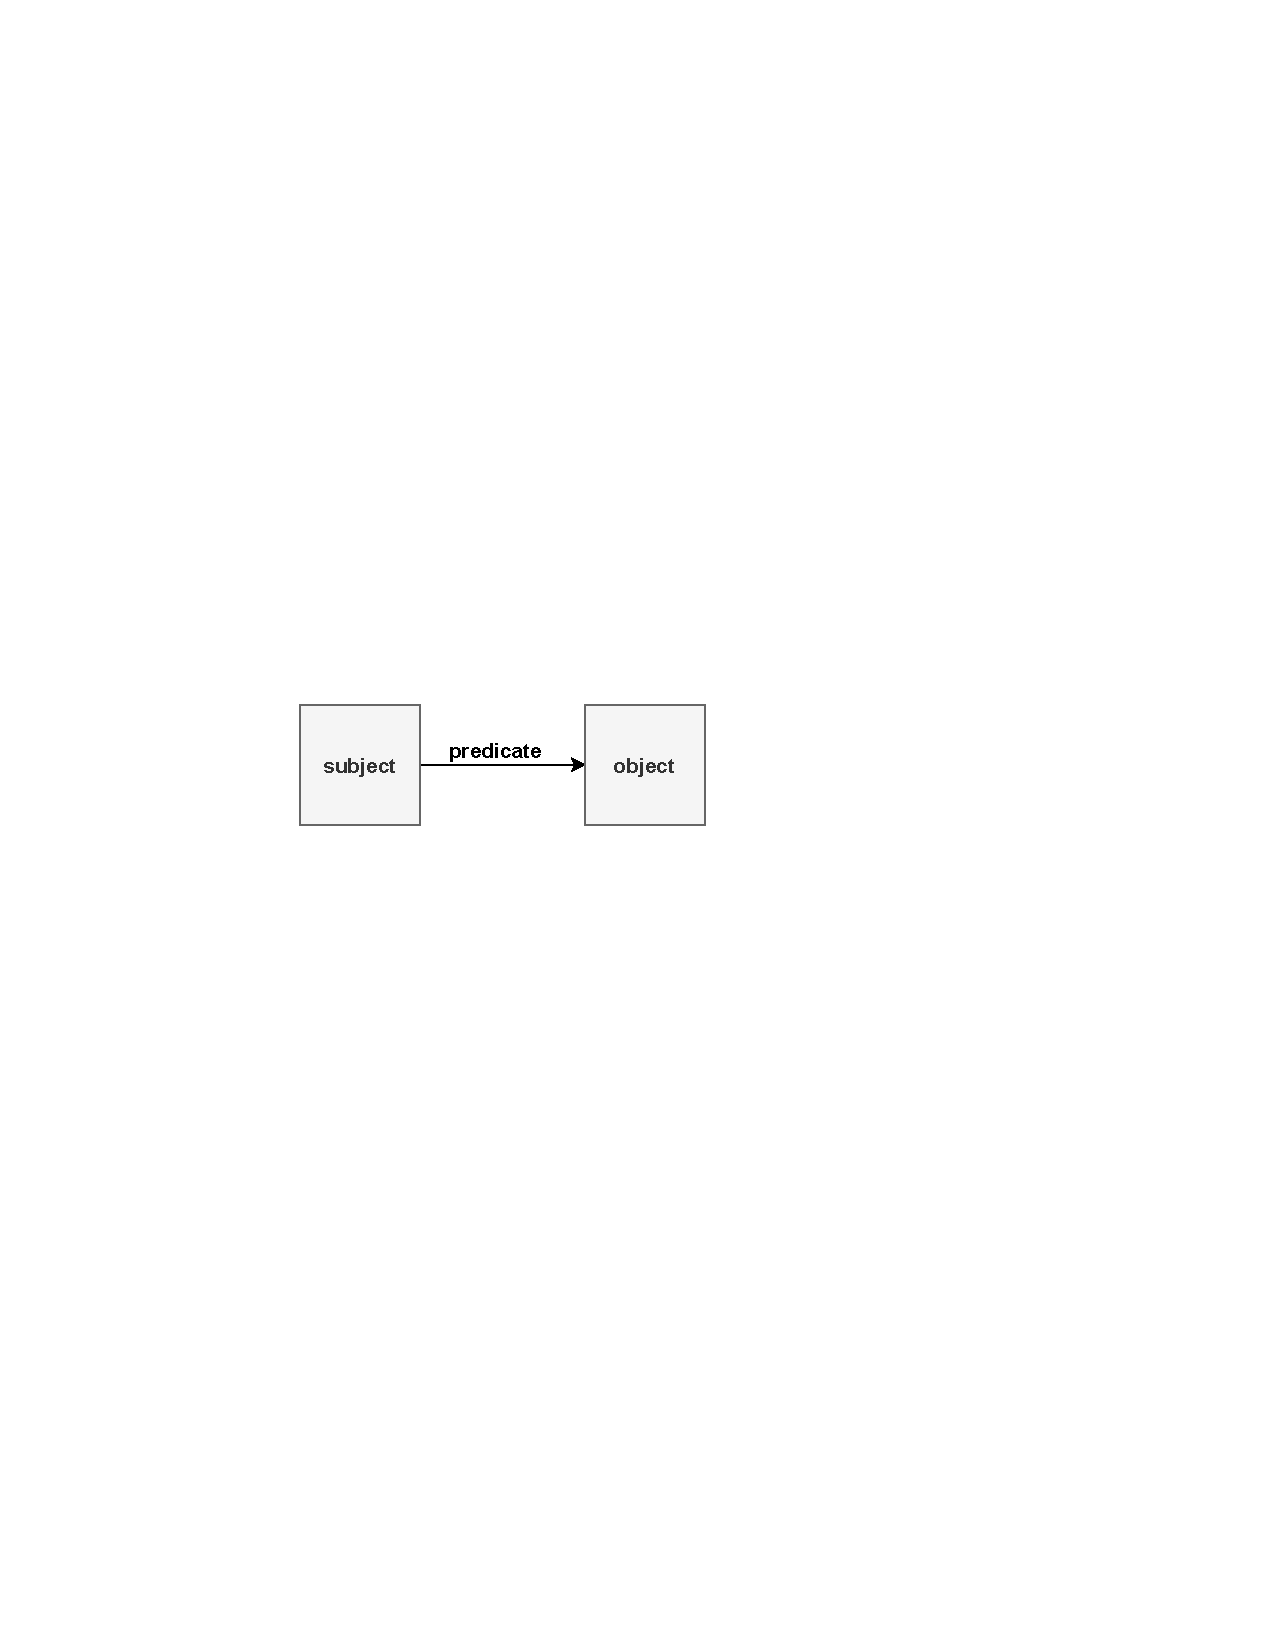
\includegraphics[trim=5cm 14cm 9.5cm 12cm]{images/rdf-ex1.pdf}
    \caption{A triple}
    \label{fig:RDF-ex1}
\end{figure}


\section{OWL}
The Web Ontology Language (OWL) is the standard ontology language for RDF~\cite{OWL_W3C}. OWL 2 is the newest version\footnote{https://www.w3.org/TR/owl2-overview/} OWL combines Description Logics (DL) expressiveness with RDF technology. It is the recommended language to use to express ontologies. An ontology defines the concepts in a domain and the relationship between the classes and the properties.\footnote{https://www.w3.org/standards/semanticweb/ontology}

An OWL ontology defines the concepts and properties and their relationships, by using a set of axioms. So an OWL ontology is a set of axioms which restrict the classes and properties, and the types of relationships permitted between them.
With an OWL ontology we then can apply reasoning on the dataset we have and infer additional information based on the data and axioms that we have.\footnote{https://en.wikipedia.org/wiki/Web\_Ontology\_Language} 
OWL reasoning on a lot of data is very expensive, so it's not always done. 
For example, if we have an axiom that states that every horse is an animal, and we have a RDF triple in our dataset that states “Black Caviar” is a horse, then we can infer that ``Black Caviar'' is an animal. 


\section{SPARQL}
The \textit{SPARQL Protocol and RDF Query Language} is the most popular query language for RDF data. SPARQL is used to query data stored in RDF format similarly to how SQL is used to query relational data.~\cite{SPARQL_W3C} 

SPARQL is based around graph pattern matching which is a mechanism where we can create a subgraph of the RDF graph by assigning values to variables in the graph. Every variable and blank node in a pattern will be mapped to a resource, a blank node, or a literal in the RDF graph.

\textit{Basic Graph Patterns (BGP), Group Graph Patterns, Filters or Constraints and Optional Graph Patterns} are some of the different types of graph patterns. 

A BGP is a set of RDF triples or an RDF graph where the subject, predicate and object can be replaced by variables. When a SELECT SPARQL query is executed over an RDF graph, the query will return all possible combinations of values for the variables in the BGP, such that the triples in the BGP occurs in the RDF dataset. Then the graph pattern will actually match and assign values to the defined variables which matches a subgraph of the RDF graph. The executed query will return a solution as long all the BGPs in the query are matched.

\section{Data Access Systems}
\subsection{Visual Query Systems} \label{Visual Query Systems}
A data access system is a system that allows a user to access and interact with data~\cite{vidar-phd-2020}. There exists many different types of data access systems, like \textit{information retrieval systems} (IR), \textit{faceted search systems} and \textit{visual query systems} (VQS). A VQS is a system that's used to access and interact with data, similar to a database, but it uses ``visual representations to depict the domain of interest and express related requests''~\cite{VQS_for_databases}. 

As the web is expanding rapidly, and more and more people have access to the internet the volume and speed of data generation has also increased rapidly~\footnote{https://www.statista.com/statistics/871513/worldwide-data-created/}. This has lead to more and more data being available on the web to everyone. However one issue is that it's not always very easy for non-technical users to interact, query and retrieve data from the web. VQS offers a solution to this issue where the end user doesn’t have to be an expert in a query language like SQL or SPARQL~\cite{VQS_on_the_web}. An example of a VQS is \textit{OptiqueVQS}. 


\subsection{OptiqueVQS}

OptiqueVQS is an \textit{ontology-based visual query system}~\cite{OptiqueVQS_swj_article}. The project was a part of an EU project called the Optique Project.~\footnote{http://optique-project.eu/} Ontology-based visual query systems ``are systems that have access to a given domain ontology, and which use visual elements to support query construction over this domain. Such a system could, for example, show a visual representation of the partially constructed query, and present the domain implicitly by providing lists of valid modifications to the constructed query.''~\cite{vidar-phd-2020}.

One major issue with data access systems is that they require employees with great technical knowledge, so they can extract data, and employees with domain knowledge who know how to interpret and use the extracted data~\cite{VQS_search}. However, today there's usually a sharp distinction between the domain experts and technical employees~\cite{VQS_search}.

The main goal of OptiqueVQS is to provide a system which can be easily used by domain experts who have in-depth knowledge and understanding of semantics in their domain of expertise, but don't necessarily have the technical skills (i.e., constructing a complex SPARQL query). 
OptiqueVQS offers a solution which provides a ``visual query specification mechanism for users who cannot or do not desire to use formal textual query languages to retrieve data''. It's also excepted ``that domain experts with technical skills and knowledge could often benefit from the availability of such visual mechanism, particularly if they are given the opportunity to switch between textual and visual query formulation within a task.''~\cite{OptiqueVQS_swj_article}

``OptiqueVQS is a user interface to construct complex queries over data described by an ontology (See Figure~\ref{fig:optiqueVQS}). It is important for a good user experience to adjust the interface based on the available underlying data. But complex queries over large amounts of data are expensive.''~\cite{VQS_search} However this issue can be solved by using the configurations described by Vidar Norstein Klungre in the thesis \textit{Adaptive Query Extension Suggestions for Ontology-Based Visual Query Systems}.~\cite{vidar-phd-2020}


\section{Dead-End Detection and Value Suggestions}

In order to be able to do \textit{approximate dead-end detection} in an ontology-based VQS we can use an index-based framework which is based on a ``configuration structure where the classes and properties to support are given''~\cite{vidar-phd-2020}. Constructing an index for dead-end detection efficiently in an ontology-based VQS that supports ``tree-shaped, and arbitrarily large queries with typed variables and filters is not really viable''~\cite{vidar-phd-2020}. The process of calculating dead-ends perfectly would be too slow, ``since it requires the system to execute complex queries over the database after each change to the partial query.''~\cite{vidar-phd-2020}. However by using configurations we can ``determine which parts of the data to include in the index''~\cite{vidar-phd-2020}. 

The configurations that are proposed in the thesis \textit{Adaptive Query Extension Suggestions for Ontology-Based Visual Query Systems}~\cite{vidar-phd-2020} are used to determine ``both the structure of the index and how many dead-end extensions it detects, and based on this we can calculate both the precision and cost of the configuration.''~\cite{vidar-phd-2020}. The optimal configuration would be a configuration with high precision and low cost, but there's a trade off between precision and memory usage. An extensive configuration will usually lead to a high precision on dead-end detection while requiring a really memory heavy index, and a limited configuration will usually lead to a low precision on dead-end detection while being really cheap memory wise. Another issue is that finding the optimal configuration with the highest precision and low cost is a non-trivial combinatorial optimization problem. A solution to this problem is proposed by Vidar Norstein Klungre~\cite{vidar-phd-2020} where ``a set of different configuration generation methods that use efficient cost and precision estimates and search heuristics''~\cite{vidar-phd-2020} can be used to produce useful configurations. 

The main idea behind the framework ``is to define an index that stores precomputed answers of queries that use the most central classes and properties of the ontology or navigation graph. If the query the system needs to execute in order to detect dead-ends is covered by this index, then it can retrieve answers efficiently directly from the index, and use the answers to find and present all dead-ends. But, if the query is not covered by the index, then the system needs to prune it until the remaining part can be answered by the index. When the system has to prune the query, it may fail to detect some dead-ends, but, by selecting what to index in a clever way, the approximation will give very good results.''~\cite{vidar-phd-2020}. By ignoring ``the less important parts of the partial query when computing dead-ends'' we will ``limit the number of joins that needs to be pre-computed, which means that efficient results can be computed with the use of a finite index.''~\cite{vidar-phd-2020}. It's been proven theoretically in the thesis~\cite{vidar-phd-2020} that this framework can be used to ``construct an efficient index based on the configuration query and the dataset, and that this index returns the same results as the dataset to pruned queries''~\cite{vidar-phd-2020}

\section{Search Engine}
\subsection{Elasticsearch}


\section{Research plan}
The first step is to implement the faceted filtering based on a Elasticsearch index. This entails implementing and integrating the index construction and index component with OptiqueVQS, and also implementing the communication between the frontend and backend. After implementing and integrating the dead approximate dead-end detection, we'll focus on setting up, configuring and managing the Elasticsearch clusters to scale our system for better performance and stability. Then we'll do experimental and comparative evaluation of the approach on large data sets. 

Lastly if time permits, then the work can be extended in several directions. We can implement text input completion based on search technology. We can also experiment with other no-SQL storage engines, like e.g. MongoDB. Storing the extension index in either a relational database or a search engine is not very memory efficient, but these two approaches are very scalable. But we believe document-oriented databases like MongoDB can be more memory-efficient since it can be more suitable for tree-shaped structures like the configuration structure~\cite{vidar-phd-2020}.   

\section{RDFS, Turtle, Search Engine, ES, RDFox, Datastore, Navigation graph?????}

\chapter{Design}

\section{Search engine}
We will store the precomputed answers of queries that use the most central classes and properties of the ontology in an index so we could efficiently detect dead-ends. So we would need a technology that we can use to store the index, find if an executed query is covered by the index, and retrieve answers efficiently directly from the index. As mentioned in Section \ref{Problem description} we want to store the index in a search engine since the queries to the index only concern a single table. By using a search engine we can scale up the index storage over a cluster and increase the performance, in addition to using typical search engine features like text input completion.

In Section \ref{Visual Query Systems} we mentioned that information retrieval system is a type of a data access system. ``Information retrieval (IR) is finding material (usually documents) of an unstructured nature (usually text) that satisfies an information need from within large collections (usually stored on computers).''~\cite{IR_book}. A search engine is an application of IR techniques that's used to find information on the web~\cite{IR_and_SE}.

Before looking at all the available search engines that exists and that we could use for our project, we need to first to define what features and properties we are looking for. Software license is really important since we will integrate the search engine to OptiqueVQS. By not considering or even choosing a very restrictive license then it could be a huge issue when we would publish OptiqueVQS. \textit{Proprietary software} and \textit{free and open-source software} (FOSS) are the two most common categories for software under copyright law\footnote{https://en.wikipedia.org/wiki/Software\_license}. So we should only look for search engines with FOSS license, but we also need to be sure which rights a license grants. Just because a license is a FOSS license doesn't mean that the license grants all rights to the developers. For example the MIT license is a permissive license which has very limited restrictions on reuse~\footnote{https://en.wikipedia.org/wiki/MIT\_License}, while the GPL license is a copyleft license with a bit more restrictions than the MIT license. With the GPL license any derivative work has to be distributed under the same or equivalent license terms~\footnote{https://en.wikipedia.org/wiki/GNU\_General\_Public\_License}. 

In Section~\ref{Problem description} it was mentioned briefly that dead-end detection is acutally a quite common feature in faceted search systems by using index-based search engines like Lucene. These systems use facets which are a subset of filtering, that allows the users to for ``objects of a given class by applying filters to independent properties of the class''~\cite{vidar-phd-2020}. The limiting factor with faceted search systems is that the queries can only ask for objects to one particular class. So the ``queries generated by faceted search systems must contain exactly one variable typed to the selected class, and this variable can only be connected to at most one variable for each facet''~\cite{vidar-phd-2020}. Only queries without any joins in the context of SQL are allowed in these systems. Adaptive features that help the users to select useful filters are very common in facted search systems since they usually improve the user experience. One such feature is dead-end detection, where ``dead-ends are usually disabled or removed entirely, in order to prevent the user from selecting them''~\cite{vidar-phd-2020}

The index construction process and how we can use the index correctly is explained in depth in the thesis \textit{Adaptive Query Extension Suggestions for Ontology-Based Visual Query Systems}~\cite{vidar-phd-2020}. We have also explained why faceted search systems won't work with more expressive queries that queries over multiple classes since the predefined schema limits both the queries and the dataset. However we will actually implement the dead-end detection by using a faceted search system. The simplest way to implement the dead-end detection that ensures sufficient efficiency is by using the state-of-the-art faceted search systems. This can be done because the both the index and queries are limited by the variables and structure of the configuration query Z. A configuration query Z is a simple, filterless query that is legal with respect to the navigation graph.~\cite{vidar-phd-2020} 
So ``we can turn our configuration-based solution into standard faceted search by considering every data property in Z to be a facet of the root''~\cite{vidar-phd-2020}. State-of-the-art search systems are usually known for their efficiency and scalability. For example, Linkedin have over 750 million users and over 50 million registered companies. They allow users to search for other registered users and companies by using faceted search. So by using a search engine to store the index in a search engine, we can guarantee both sufficient efficiency and scalability.

We looked at many search engines like Splunk, MarkLogic, Sphinx, Algolia, Microsoft Azure Search, Lemur, Manatee, Terrier Search Engine, Amazon CloudSearch, Xapian, Elasticsearch and Solr. Most of these search engines lacked some of the core features and properties that we are looking for. For example Microsoft Azure Search, Amazon CloudSearch, Splunk and MarkLogic aren't open source. Algolia is open source however it's not free. Manatee, Terrier Search Engine and Xapian all have FOSS license however they also have subpar documentation and small community. 

In the end the two best options for our case were Elasticsearch and Solr. Both of these search engines are based on the Lucene library. Both of these search engines are very similiar feature wise. Both are free and open source, with permissive license. They both support faceted search and other additional search engine features like text input completion. Perfomance and scalability is also very good with both engines. We compare Solr with Elasticsearch in Table~\ref{tbl:solarVsElastic}. However in the end we decided to choose Elasticsearch because of two main reasons. Elasticsearch has better inherent scalability, the search engine has been designed from the ground up to be scalable, and for that reason it have better support for scaling and cluster management. Elasticsearch is the most popular search engine and the community is much larger than the Solr community. So there's a lot more guides, tools and examples about Elasticsearch than Solr. Besides the guides on the internet the Elasticsearch documentation is more mature and better organized and easier to use than Solr's documentation. 

\begin{table}[]
\begin{tabular}{|l|l|l|}
\hline
\textbf{}                                                                    & \textbf{Solr}         & \textbf{Elasticsearch}  \\ \hline
\textbf{License}                                                             & Apache License 2.0    & Elastic License or SSPL \\ \hline
\textbf{\begin{tabular}[c]{@{}l@{}}Popularity \\ (DB-engines)\end{tabular}}  & 3                     & 1                       \\ \hline
\textbf{Open Source}                                                         & Yes                   & Yes                     \\ \hline
\textbf{Documentation}                                                       & Decent                & Good                    \\ \hline
\textbf{\begin{tabular}[c]{@{}l@{}}Server Operating \\ Systems\end{tabular}} & All OS with a Java VM & All OS with a Java VM   \\ \hline
\textbf{APIs}                                                                & Java API and REST API & Java API and REST API   \\ \hline
\textbf{Faceted Search}                                                      & Yes                   & Yes                     \\ \hline
\textbf{\begin{tabular}[c]{@{}l@{}}Autocomplete \\ suggestions\end{tabular}} & Yes                   & Yes                     \\ \hline
\textbf{\begin{tabular}[c]{@{}l@{}}Learning Curve \\ and \\ Ease of Use\end{tabular}} &
  \begin{tabular}[c]{@{}l@{}}Overall, more difficult to \\ set up and manage. Both \\ of these technologies are \\ quite easy to begin \\ working with. But \\ Elasticsearch is much \\ easier to take into \\ production and scale\end{tabular} &
  Easier to set up and scale \\ \hline
\textbf{Cache} &
  \begin{tabular}[c]{@{}l@{}}Global, invalidated with \\ each segment change\end{tabular} &
  \begin{tabular}[c]{@{}l@{}}Per segment, better for \\ dynamically \\ changing data\end{tabular} \\ \hline
\textbf{Data Sources} &
  \begin{tabular}[c]{@{}l@{}}Solr supports over a \\ thousand file types \\ using the Apache \\ Tika library, and it has \\ request handlers for a \\ number of popular file \\ types such as CSV, \\ Word docs, \\ PDF, and XML.\end{tabular} &
  \begin{tabular}[c]{@{}l@{}}Elasticsearch uses \\ JSON to ingest data \\ from multiple \\ sources. Elasticsearch \\ can also use the \\ Apache Tika library \\ to support rich documents.\end{tabular} \\ \hline
\textbf{Performance}                                                         & High                  & High                    \\ \hline
\textbf{Scalability} &
  \begin{tabular}[c]{@{}l@{}}Support from Solr Cloud \\ and Apache Zookeeper \\ dependence for \\ cluster coordination\end{tabular} &
  \begin{tabular}[c]{@{}l@{}}Better inherent scalability; \\ design optimal for \\ cloud deployments\end{tabular} \\ \hline
\end{tabular}
\caption{Comparison table between Solr and Elasticsearch}
\label{tbl:solarVsElastic}
\end{table}

\newpage
\section{Architecture}
The next step after deciding the search engine is how will we implement the communication between the frontend and the backend. We already know that we need to implement a component which handles the construction of the index and stores it in Elasticsearch. In addition to a component which will handle the use of the index. This component will retrieve the results from Elasticsearch and prepare the results before sending the final result to the frontend.

Regarding the communication between the frontend and the bakcend, we though about two different implementations that would work. The first option is where the frontend would directly send queries to Elasticsearch (ES) by using ES REST API. The second approach is to send the queries to the index use component (See Figure~\ref{fig:optiqueVQS_architecture}). In the end we decided to use the second approach since with the first approach we then need to store the configuration structure in the frontend to be able to do query prunning. To be able to send the queries to ES we also need to transform the queries into a valid ES JSON query. The second approach would be simpler, more efficient, more modular and easier to scale. We'll just extend the index use component to do query prunning and then send the query to ES. The configuration structure is already stored in the backend since it's used for the index construction process. So we wouldn't need to store the same configuration both in the frontend and the backend. It would also save us the hassle of needing to update the configurations both in the frontend and backend each time the configuration structure is updated. The dead-end detection process wouldn't be limited by the frontend, so we could still detect dead-ends even if most of the frontend is changed as long the frontend sends queries to the index use component.

We also decided on what's the best data format of the queries that the frontend sends to the index use component. We though about three different data formats, which are graph structure, SPARQL and SPIN. In the end we decided with using sending the query as a graph structure. The easiest and fastest format would be graph structure since we already store the queries in OptiqueVQS as a graph structure. With this format the frontend doesn't have the troubles of parsing and serializing the queries. It would also requires less communication between the frontend and backend, but the graph structure we are using isn't some standard query format like SPARQL. So SPARQL would be better if we would like to extend our backend to support other frontends or if the graph structure is largely updated in the future. SPIN is a RDF representation of SPARQL where the main benefit of SPIN is that it's possible to consistently store SPARQL queries together with the domain model, since it provides an alternative representation of SPARQL queries beyond the textual format~\cite{SPIN_W3C}. 

\begin{figure}[htp]
    \centering
    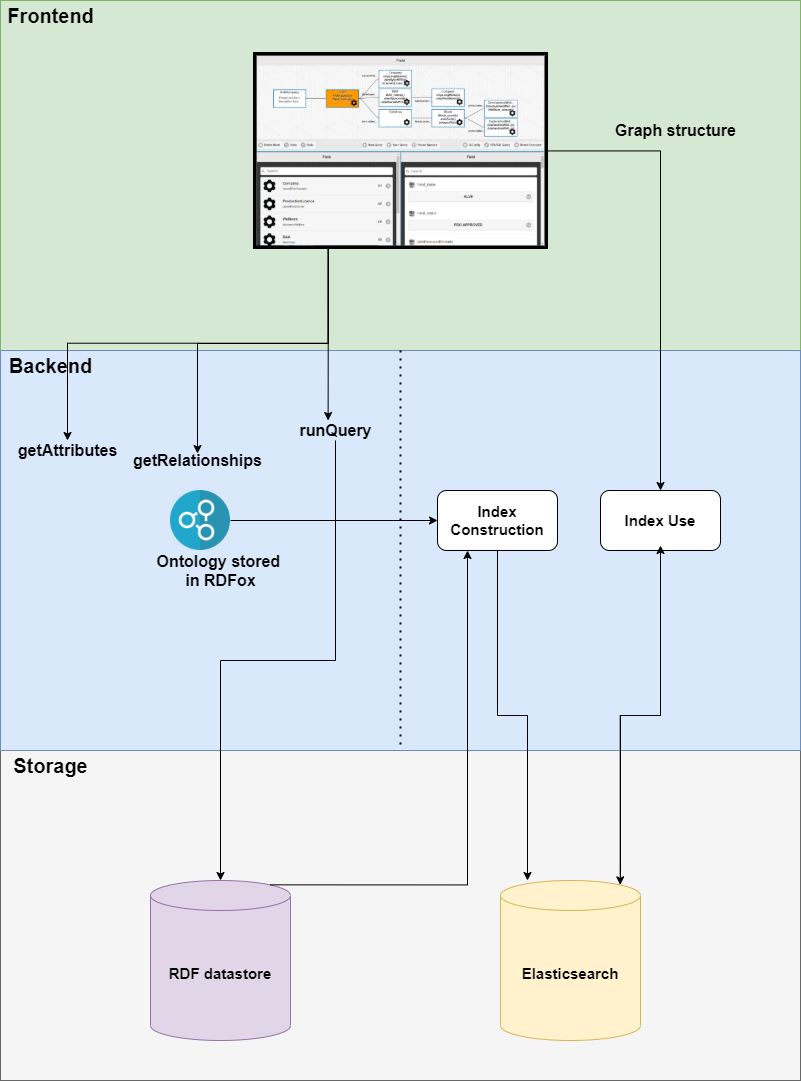
\includegraphics[width=12cm]{images/master-arch.png}
    \caption{OptiqueVQS architecture}
    \label{fig:optiqueVQS_architecture}
\end{figure}

\chapter{Implementation}

\chapter{Evaluation}

\chapter{Conclusion and Future Work}
\section{Conclusion}
\section{Limitations}
\section{Future Work}


\newpage
\Urlmuskip=0mu plus 1mu\relax
\bibliographystyle{plain}
\bibliography{references.bib}
\end{document}
